\section{Introduction}
This \lcnamecref{chap:nmp} presents a framework for passing messages between discrete points on a finite lattice, where each point updates its internal data (and thus the messages it sends) based on messages received.  Each point is uniquely connected to other points and so has its own \emph{neighbourhood}, being the specific other points it communicates with.  A key aspect of this \emph{\gls{nmp}} computation is that the messages to a given neighbour depend upon the messages received previously from \emph{all} neighbours, \emph{except} the neighbour to which the current message is sent.    This necessarily means that in \gls{nmp} each grid location must have at least two neighbours.  A single neighbour cannot form a meaningful neighbourhood.  This \lcnamecref{chap:nmp} focuses on the \emph{square lattice} but, \gls{nmp} applies equally to lattices of any shape, dimension or connectivity.

For the purposes of this \lcnamecref{chap:nmp}, the individual computational units in the lattice are termed \emph{\glspl{pe}}.\footnote{The short form ``\gls{pe}'' is derived from ``processing element'' in the same way that ``pixel'' is derived from ``picture element''.}  These are the logical base units for computation for current purposes and are represented by \gls{cps} \glspl{tlc}.  A visual example of the \gls{nmp} process for the \emph{\gls{fne}} on the square lattice is shown in \cref{fig:nmp:gridmessaging}.  A \gls{pe} in the grid received messages from its neighbours to the left, right, and bottom at generation \(t - 1\), and has used the data from those messages in preparing its new message to be sent to the neighbour above at iteration \(t\).  The same is performed for each other neighbour too.

\begin{figure}
    \centering
    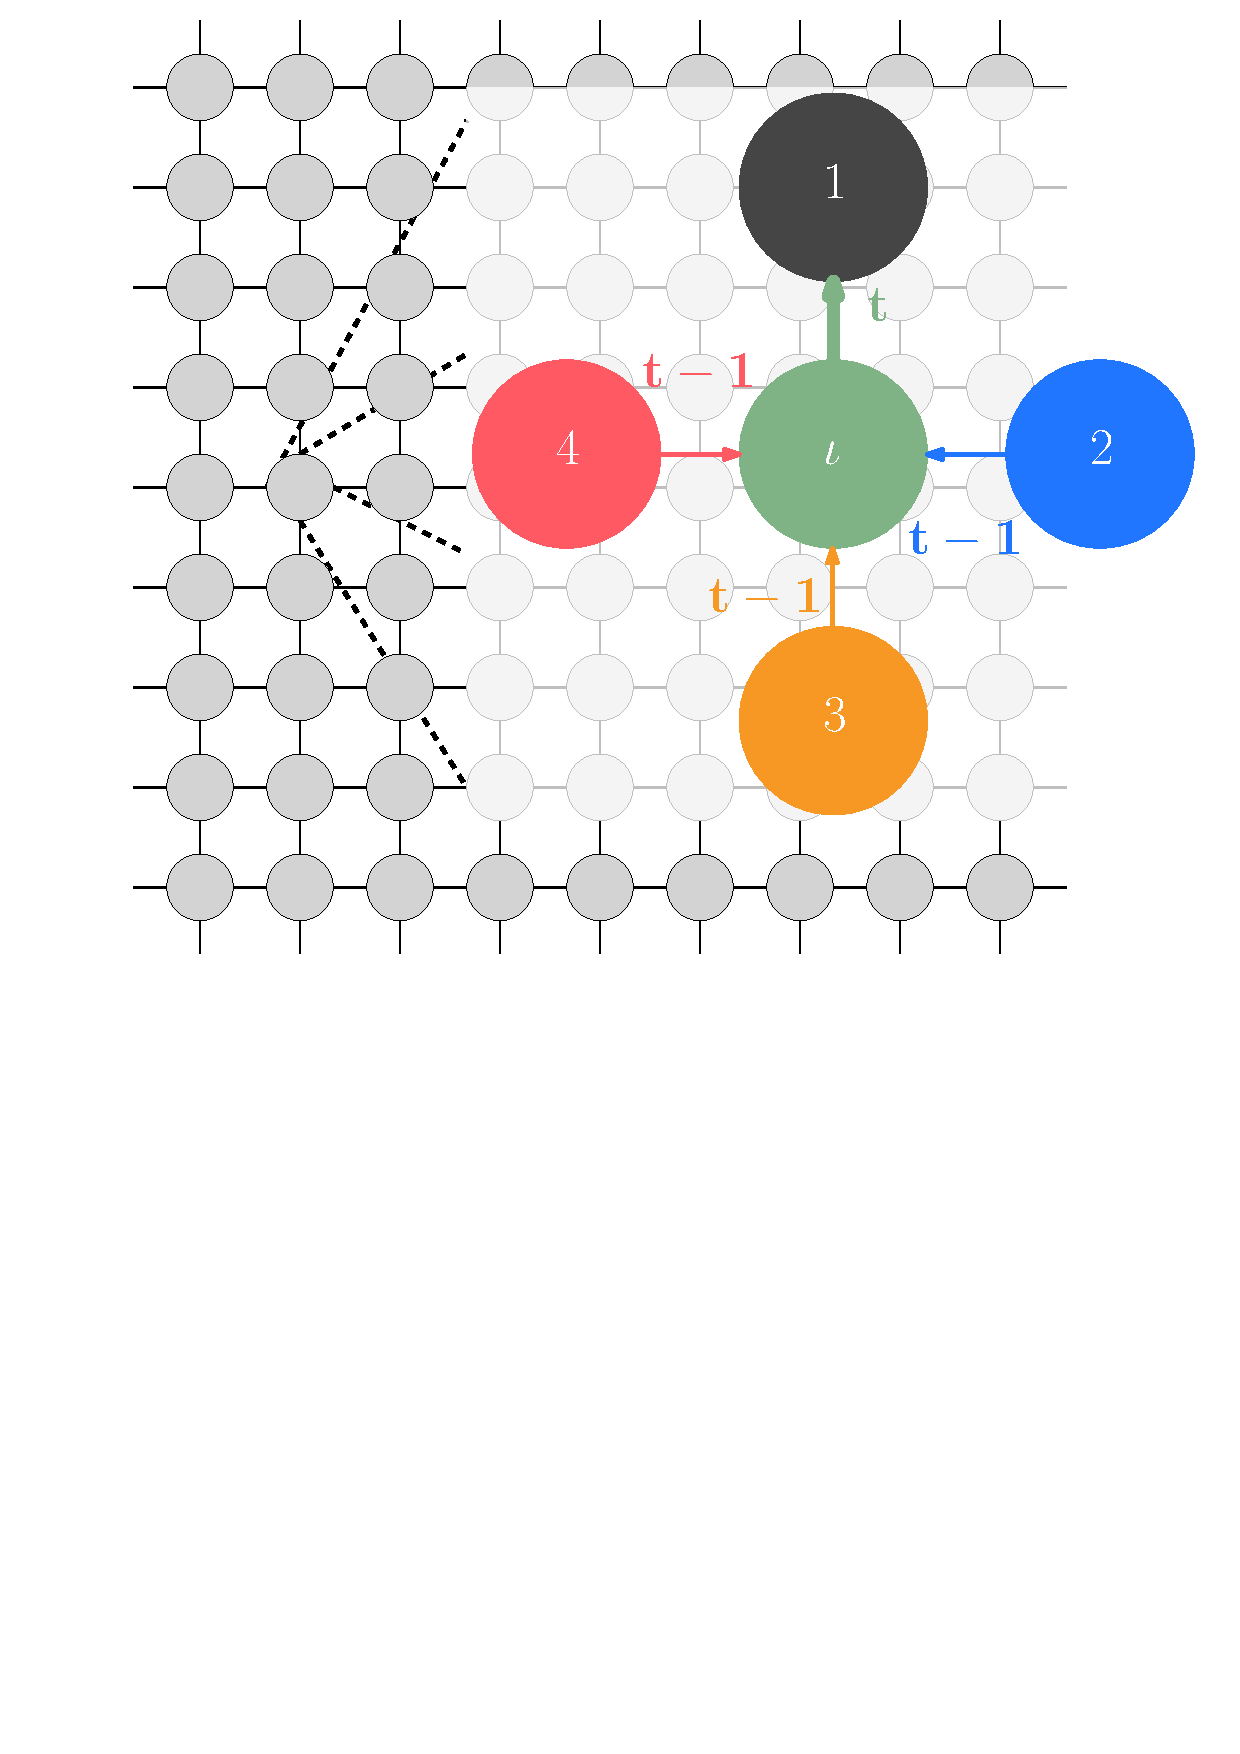
\includegraphics[keepaspectratio,width=1.0\linewidth]{chapters/nmp/images/bp_diagram_recoloured_iotacentre.pdf}
    \caption[Diagram of the central concept of \gls{fne} \glsxtrlong{nmp} on a grid]{Diagram of the central concept of \gls{fne} \gls{nmp} on a grid \cite{lbpmpsmpic}.  Each circle represents a \gls{pe}, labelled following the pattern of \cref{fig:nmp:iota_proxels_environment_oracle}.  The central \gls{pe} \(\iota\) needs to compute a new message to send at time \(t\) to the \gls{pe} \(1\) above it, so it performs a computation to combine the results of the messages received from the other three neighbouring cells (\(2\), \(3\) \& \(4\)) at time \(t - 1\) (indicated by the thin and fat arrows).  The same is applied to every other neighbour, too.}
    \label{fig:nmp:gridmessaging}
\end{figure}

Conceptually, there are two distinct aspects of the \gls{nmp} process.  The message passing itself, which occurs externally to \glspl{pe} over channels connected to other \glspl{pe}, and the data/message updates, which occur internally.  The focus of this \lcnamecref{chap:nmp} is the external side, and it uses communication with an oracle to represent the internal computation, which is largely orthogonal to the inter-\gls{pe} communication.

There are (at least) two separate ways to model the \glspl{pe}' communication:  a \emph{\gls{gs}} system-wide view, where the states and steps taken occur across the system as a whole and every \gls{pe} carries out its operations simultaneously according to the same rules.  Or, a per-\gls{pe} view, where each \gls{pe} has its own state and advances \emph{asynchronously}\footnote{Recall from \vref{sec:back:syncasync} that the idea of asynchronicity used here follows the traditional concept from distributed computing, and so is \emph{different} to that sometimes used in other \gls{ps}.} without regard to others' objects, states, and rulesets.  This \lcnamecref{chap:nmp} explores both and finds in the process that an intermediate third, \emph{\gls{ls}}, model arises naturally as a hybrid of the other two.

The modelling and implementation of \gls{nmp} proves unexpectedly challenging.  On the surface, it seems as if it should be a straightforward problem, and in the synchronous (hereafter \emph{\gls{gs}}) form (\cref{sec:nmp:systemwide}) it \emph{is} reasonably simple.  It requires only nine rules, most of which have exactly one term on both the left-hand- and right-hand-sides and none of which use \glspl{promoter} or \glspl{inhibitor} (see \cref{chap:cpsystems} for more on these concepts).

% The challenge arises in modelling the asynchronous version.  The possibility of messages for the same iteration arriving at separate times necessitates bookkeeping.  There is a need to track from which neighbours messages have been received for a given generation to decide which neighbours the \gls{pe} is now ready to send a new message to.  This gives rise to inescapable complexity and opens up the undesirable possibility of deadlock through an unsuitable design.

The challenge arises in modelling the asynchronous version.  The possibility of messages for the same iteration arriving at separate times necessitates bookkeeping.  It is necessary to track the sending neighbour from which each message for a given generation is received, to decide which neighbour(s) the current \gls{pe} is now ready to send a new outgoing message.  This gives rise to inescapable complexity and opens up the undesirable possibility of deadlock through an unsuitable design.

This \lcnamecref{chap:nmp} begins with describing a straightforward \gls{gs} \gls{nmp} system.  Then, it provides an asynchronous \gls{pe}-specific version of the same, followed by an adaptation of the asynchronous system to a \gls{ls} system. Next is a short example of a potential evolution of the asynchronous system to clarify the expected operation of the system.  Lastly, this \lcnamecref{chap:nmp} analyses the asynchronous system and reports the results of comparative computer experiments for all three systems.  The analysis proves that the asynchronous system sends precisely the same number of messages as the \gls{gs} system (one per generation per neighbour) but that the data used to compute new messages may vary slightly depending on the ordering of messages received.  Furthermore, the empirical results verify the operation of the asynchronous system and support the hypothesis that the \gls{ls} and asynchronous systems are faster than an equivalent \gls{gs} version.

\subsection{Belief Propagation}

This \lcnamecref{chap:nmp} was originally motivated by attempts to model \emph{\gls{lbp}} for \gls{sm} (see \eg{} \cite{Blake2011,Felzenszwalb2011,JianSun2003}) in \gls{cps}.  \emph{\Gls{bp}} was originally introduced to solve inference problems in AI on graphs \cite{Pearl1982} by treating the nodes as communicating objects, which passed messages backwards and forwards, updating their outgoing messages based on the incoming ones, to solve the problem.  The original formulation relied upon the graphs having a tree structure, however.  Each node would receive a message from its parent, pass that to its children, receive new messages back from the children and pass its own newly computed message back to its parent based on those received from the children.

In the case of \gls{sm}, the output is a (typically rectangular) grid representing an output image.  This means that the computation, sited on this grid, is inherently non-tree-structured.  Instead, each output node is connected to its neighbours -- usually the \gls{fne} -- which means that messages travel in loops on the grid.  To deal with this situation, \gls{bp} was adapted to \gls{lbp}, which was first applied to \gls{sm} by \citeauthor{JianSun2003} \cite{JianSun2003}.  The algorithm was then significantly improved upon by \citeauthor{Felzenszwalb2006} \cite{Felzenszwalb2006}.

\Gls{nmp}, as described in this \lcnamecref{chap:nmp}, can simulate \gls{lbp} effectively, and \cref{sec:nmp:example,sec:nmp:analysis,sec:nmp:experiments} focus on the \gls{fne}.  The main change required is to replace the oracle with appropriate computations for \gls{bp} \gls{sm}.  \Gls{nmp} can be generalised further, however, to perform other computations or use other communication arrangements besides the \gls{fne}.  While this work was originally inspired by \gls{lbp}, it is a generic framework for \emph{any} computations that may be modelled with communication on a lattice, when the outgoing message to one neighbour depends on the messages received from other neighbours.